\documentclass[border=4pt]{standalone}
\usepackage{amsmath,amssymb,amsfonts}
\usepackage{xcolor,colortbl,array,booktabs,multirow}
\usepackage{tikz}
\usepackage{pgfplots}
\pgfplotsset{compat=1.16}
\usetikzlibrary{arrows, automata, backgrounds, calendar, chains, decorations,
    matrix, mindmap, patterns, petri, positioning, shadows, shapes.geometric,
    trees, shapes, decorations.pathreplacing, calc, tikzmark, arrows.meta,
    intersections, fit, graphs, quotes, angles, decorations.markings}
\newcommand{\st}{\text{ s.t. }}
\newcommand{\x}{\mathbf{x}}
\renewcommand{\b}{\mathbf{b}}
\renewcommand{\c}{\mathbf{c}}
\newcommand{\A}{\mathbf{A}}
\newcommand{\y}{\mathbf{y}}
\newcommand{\z}{\mathbf{z}}
\newcommand{\R}{\mathbb{R}}
\newcommand{\RR}{\mathbb{R}}
\newcommand{\Z}{\mathbb{Z}}
\newcommand{\ZZ}{\mathbb{Z}}
\newcommand{\npcomplete}{NP-complete}
\providecommand{\true}{\text{TRUE}}
\providecommand{\false}{\text{FALSE}}
\tikzset{vertex/.style={circle,fill=black!25,minimum size=20pt,inner sep=0pt},
    edge/.style={draw,thick,-},weight/.style={font=\small},
    selected vertex/.style={vertex, fill=red!24},
    selected edge/.style={draw,line width=2pt,-,red!50},
    ignored edge/.style={draw,line width=2pt,-,black!20}}
\newcommand{\vect}{\vec}
\providecommand{\ds}{\displaystyle}
\providecommand{\longvect}{\overrightarrow}
\usepackage[normalem]{ulem}
\definecolor{ocre}{RGB}{243,102,25}
\providecommand{\leftB}{\left[}
\providecommand{\rightB}{\right]}
\tikzset{directed/.style={postaction={decorate,decoration={markings,mark=at position .65 with {\arrow{>}}}}},
    directed1/.style={postaction={decorate,decoration={markings,mark=at position .65 with {\arrow{>}}}}}}
\begin{document}
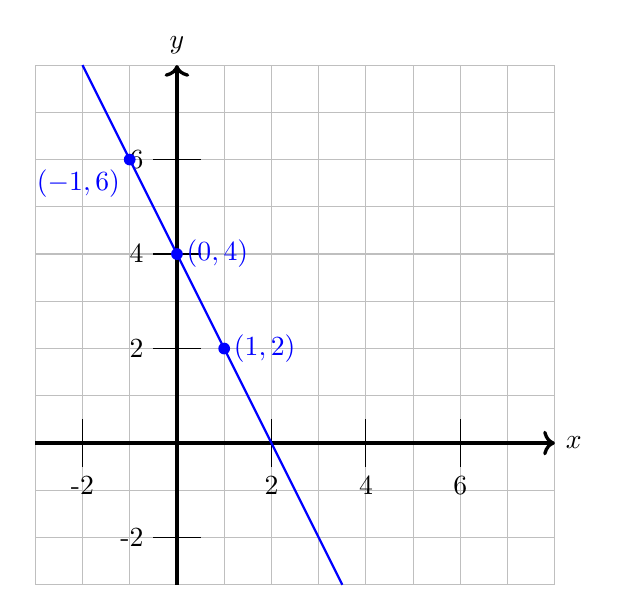
\begin{tikzpicture}[scale = 0.6]
    % Grid and axes
    \draw[gray!50, thin, step=1] (-3,-3) grid (8,8);
    \draw[very thick,->] (-3,0) -- (8,0) node[right] {$x$};
    \draw[very thick,->] (0,-3) -- (0,8) node[above] {$y$};

    % Axis labels
    \foreach \x in {-2,2,4,6} \draw (\x,0.5) -- (\x,-0.5) node[below] {\x};
    \foreach \y in {-2,2,4,6}  \draw (0.5,\y) -- (-0.5,\y) node[left] {\y};

    % Vertices
    \node[blue] at (-1,6) [circle,fill,inner sep=1.5pt]{};
    \node[blue] at (0,4) [circle,fill,inner sep=1.5pt]{};
    \node[blue] at (1,2) [circle,fill,inner sep=1.5pt]{};
    

    % Labels for vertices
    \node[blue,anchor=north east] at (-1,6) {$(-1,6)$};
    \node[blue,anchor=west] at (0,4) {$(0,4)$};
    \node[blue,anchor=west] at (1,2) {$(1,2)$};
    
    \draw[blue, thick] (-2,8) -- (3.5, -3);
\end{tikzpicture}
\end{document}
